\documentclass[11pt,compress,serif]{beamer}
%\includeonlyframes{current}

\usepackage[utf8x]{inputenc}
\usepackage[T1]{fontenc}
\usepackage[english]{babel}
% \usepackage{booktabs}
\usepackage{hyperref}
\usepackage{url}
%\usepackage{auto-pst-pdf}
%\usepackage{pst-plot}

% \usepackage{pstricks-add}

\usepackage{graphicx}
\definecolor{mygreen}{HTML}{4A7023}

\usepackage{xspace}
\usepackage{xcolor}
\usepackage{minted}
\definecolor{rulecolor}{rgb}{0.80,0.80,0.80}
\newminted{python}{frame=single,rulecolor=\color{rulecolor}, fontsize=\scriptsize}

\graphicspath{{./images/}}

\DeclareMathOperator{\Tr}{Tr}
\DeclareMathOperator{\E}{E}
\DeclareMathOperator{\Var}{Var}

% Theme
\mode<presentation>
{
    \usetheme{default}
}

\setbeamertemplate{footline}[frame number]


% Non navigation symbal
\setbeamertemplate{navigation symbols}{}

% Between section
\AtBeginSection[]
{
    %   \frame
    %   {
    %       \frametitle{Outline}
    %       \tableofcontents[currentsection]
    %   }
}

% Between subsection
\AtBeginSubsection[]
{
    %   \begin{frame}<beamer>
    %    \frametitle{Outline}
    %    \tableofcontents[currentsection,currentsubsection]
    %   \end{frame}
}


% Talk information
\author[A. Joly]{Arnaud Joly}
\title{The genesis of clusterlib \\A open source library to tame your favourite super-computer}
% \institute[Ulg]{\includegraphics[height=2cm]{logo_coul_texte_blason_cadre}}
\date{May 2015}
\subject{}
%\logo{} %change here. I used an eps file logo, you can use jpg or other format


\begin{document}
    
\frame[plain]
{
    \titlepage
}

\frame{

\frametitle{Use case for the birth of clusterlib}
\framesubtitle{Solving supervised learning tasks}
The goal of supervised learning is to learn a function from
\structure{input}-\alert{output} pairs in order to predict the \alert{output} 
for any new \structure{input}.

\begin{footnotesize}
    \begin{columns}[b]
        \begin{column}{0.5\textwidth}
            \begin{block}{}
                \structure{A supervised learning task}
                
                \includegraphics[width=\textwidth]{forest_pruning_nolearn}
            \end{block}
        \end{column}
        
        \begin{column}{0.5\textwidth} 
            \structure{A learnt function}               
            
            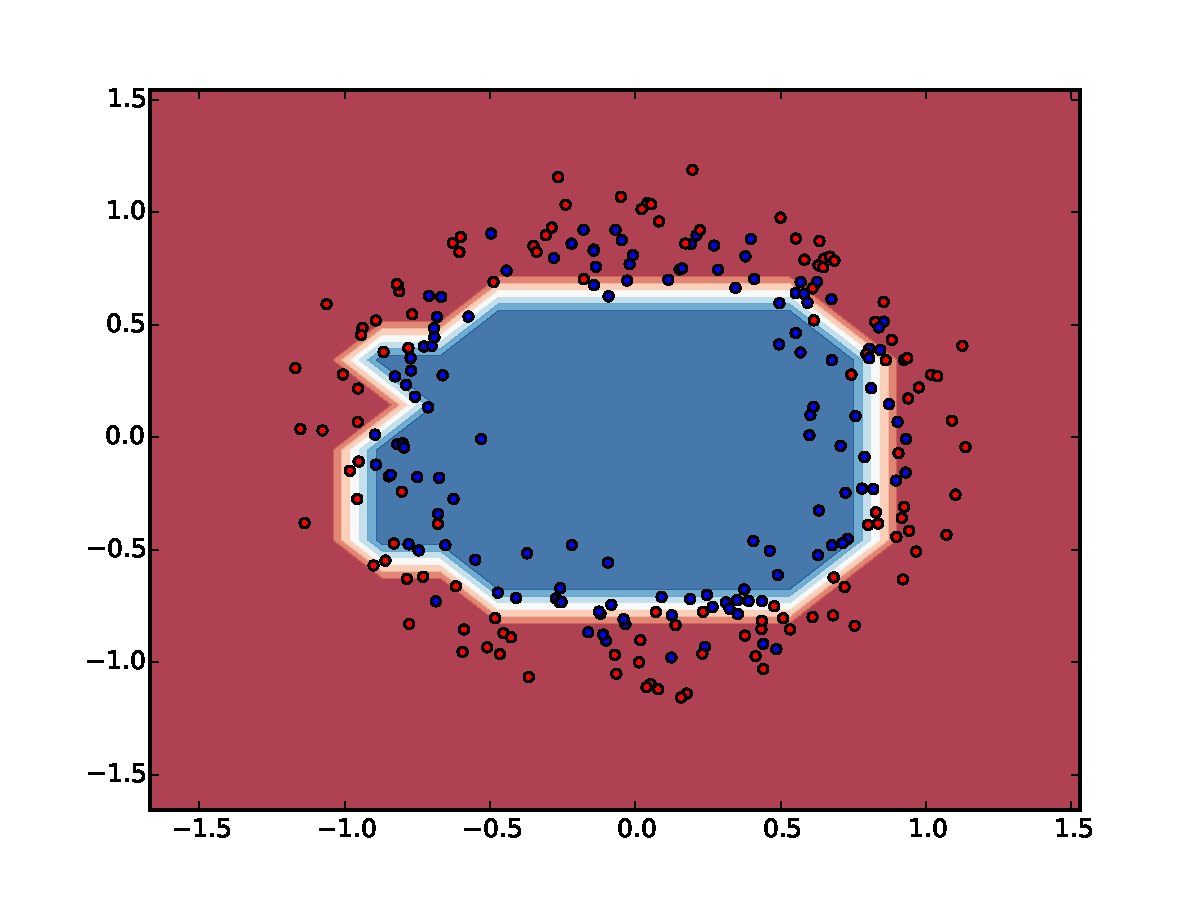
\includegraphics[width=\textwidth]{decision_tree_boundary}
            
        \end{column}
    \end{columns}
\end{footnotesize}
}

\frame{
\frametitle{Use case for the birth of clusterlib (II)}
\framesubtitle{Compression of random forest models}
The learnt function was a decision tree model. Nowadays instead of only one tree, 
we generate very large ensemble of randomized decision trees.
    
\begin{center}    
    \includegraphics[width=0.7\textwidth]{decision_tree_structure}
\end{center}

How to compress those models while preserving accuracy? 
\emph{L1-based compression of random forest models}
\cite{joly2012l1}
}


\frame{
\frametitle{Use case for the birth of clusterlib (III)}
\framesubtitle{Solving high dimensional multilabel classification tasks}

Many applications in text, biology or image processing where samples are associated 
to sets of labels or continuous response.

\begin{columns}[T]
    \begin{column}{0.5\textwidth}
        \begin{block}{Input $\mathcal{X}$ $800 \times 600$ pixel}
            \begin{center}
                \includegraphics[width=\textwidth]{image_anotation}
            \end{center}
        \end{block}
    \end{column}
    
    \begin{column}{0.4\textwidth}        
        \begin{block}{Output $\mathcal{Y}$ labels}
            driver, mountain, road, car, tree, rock, line, human, \ldots
        \end{block}
        
        \begin{block}{}
            If each label corresponds to a wikipedia article, then we have
            around \alert{4 million labels}.
        \end{block}
    \end{column}
\end{columns}

How to handle very high label space? \emph{Random forests with random projections of the output space 
for high dimensional multi-label classification \cite{joly2014random}}
}

\frame{
\frametitle{Time is running out}

I have huge set of experiments and the following upper bound

\[
O(\text{\#datasets} \times  \text{\#algorithms}  \times  \text{\#parameters}) \leq O(\text{time before deadline})
\]

But, we have \alert{embarrassingly parallel tasks}. Let's use a supercomputer. We \structure{hope} to be able  
\begin{itemize}
\item to launch easily many jobs at once ;
\item to avoid launching running or queued jobs;
\item to avoid launching completed jobs.
\item to be queue scheduler agnostic (SLURM? SGE?).
\item to have few  dependences.
\end{itemize}
  
}

\begin{frame}[fragile=singleslide]
\frametitle{A glimpse to a supercomputer user interface (SLURM)}
\framesubtitle{How to sumit a job?}

First, we need to write a bash file \texttt{job.sh} which specifies 
resources requirements (time, memory,...) 
and call the appropriate program.

\begin{minted}{bash}
#!/bin/bash
#
#SBATCH --job-name=job-name
#SBATCH --time=10:00
#SBATCH --mem=1000
srun hostname
\end{minted}

Then you can launch the job in the queue
\begin{minted}{bash}
$ sbatch job.sh
\end{minted}
\end{frame}

\begin{frame}[fragile=singleslide]
\frametitle{A glimpse to a supercomputer user interface (SLURM)}
\framesubtitle{How to check if a job is running?}

To check if a job is running, you can use the \texttt{squeue} command.

\begin{minted}{bash}
$ squeue -u `whoami`
\end{minted}

\begin{scriptsize}
\begin{verbatim}
JOBID   PARTITION     NAME       USER  ST       TIME  NODES NODELIST(REASON)
1225128      defq job-9999    someone  PD       0:00      1 (Priority)
1225129      defq job-9998    someone  PD       0:00      1 (Priority)
...
1224607      defq job-0003    someone   R    7:39:16      1 node025
1224605      defq job-0002    someone   R    7:43:25      1 node040
1224593      defq job-0001    someone   R    8:06:33      1 node035
\end{verbatim}
\end{scriptsize}



\end{frame}


\frame{
\frametitle{Back to the checklist}

\begin{itemize}
\item Can we launch easily many jobs at once? \structure{No!}
\item Can we avoid launching running or queued jobs? \structure{No!}
\item Can we avoid launching completed jobs? \structure{No}
\item Will it work for several clusters (at least SGE, SLURM)? \structure{No}
\item Do we have to install dependencies? \structure{No}, good point! 
\end{itemize}    


}


\frame{
\frametitle{Let's not reinvent the wheel}

\begin{itemize}
\item \structure{Distributed Resource Management Application API} (DRMAA): unfortunately, it's not 
       installed on all clusters (installation require root access?).  Some packages are based
       on this: \structure{python-drma}, \structure{galaxy}, \ldots
\item \structure{Bosco} (\url{http://bosco.opensciencegrid.org/}): a compatibility layer for 
       several schedulers with similar interface to SLURM/SGE.
\item \structure{FireWorks} (\url{http://pythonhosted.org/FireWorks/}): seems pretty complete, 
      but it's much more complex than my basics needs.  It also has 6 required dependencies, among 
      them mongodb, and 7 optional dependencies. 
\end{itemize}

Arf, no suitable library on the market. At this point, I decided to write clusterlib.

}

\begin{frame}[fragile=singleslide]
\frametitle{clusterlib - How to launch a job?}

First, generate a submission script on the fly
\begin{pythoncode}
>>> from clusterlib.scheduler import submit
>>> script = submit("srun hostname", job_name="test",
...                 time="10:00", memory=1000, backend="slurm")
>>> print(script)
echo '#!/bin/bash
srun hostname' | sbatch --job-name=test --time=10:00 --mem=1000 
\end{pythoncode}

Let's launch the job
\begin{pythoncode}
>>> os.system(script)
\end{pythoncode}
    
\end{frame}

\begin{frame}[fragile=singleslide]
\frametitle{clusterlib - How to launch a tons of jobs?}
    

\begin{pythoncode}
>>> for param in range(3):
...     script = submit('./main --param %s' % param, 
                        job_name='j-%s' % param)
...     print(script)
...     # os.system(script)
... 
echo '#!/bin/bash
./main --param 0' | sbatch --job-name=j-0 --time=24:00:00 --mem=4000
echo '#!/bin/bash
./main --param 1' | sbatch --job-name=j-1 --time=24:00:00 --mem=4000
echo '#!/bin/bash
./main --param 2' | sbatch --job-name=j-2 --time=24:00:00 --mem=4000
\end{pythoncode}
        
\end{frame}

\begin{frame}[fragile=singleslide]
\frametitle{clusterlib - How to avoid re-launching queued or running jobs?}
    

\begin{pythoncode}
import os
from clusterlib.scheduler import queued_or_running_jobs
from clusterlib.scheduler import submit

if __name__ == "__main__":
    scheduled_jobs = set(queued_or_running_jobs())
    for param in range(100):
        job_name = "job-param=%s" % param
        if job_name not in scheduled_jobs:
            script = submit("./main --param %s" % param,
                            job_name=job_name,
                            backend="slurm")
            os.system(script)
\end{pythoncode}

\end{frame}

\begin{frame}[fragile=singleslide]
\frametitle{clusterlib - How to avoid re-launching already done jobs?}

Firstly, record when a job is done

\begin{pythoncode}
# main.py

import sys, os
from clusterlib.storage import sqlite3_dumps

NOSQL_PATH = os.path.join(os.environ["HOME"], "job.sqlite3")

def main(argv=None):
    if argv is None: # For ease here, function parameters are sys.argv
        argv = sys.argv  
    # do heavy computation
    # Save script evaluation on the hard disk

if __name__ == "__main__":
     main()
     # Great, the jobs is done!
     sqlite3_dumps({" ".join(sys.argv): "JOB DONE"}, NOSQL_PATH)
\end{pythoncode}

\end{frame}

\begin{frame}[fragile=singleslide]
\frametitle{clusterlib - How to avoid re-launching already done jobs?}

Secondly, don't launch jobs that have already been done.

\begin{pythoncode}
# launcher.py

import sys
from clusterlib.scheduler import queued_or_running_jobs
from clusterlib.scheduler import submit
from clusterlib.storage import sqlite3_loads
from clusterlib_main import NOSQL_PATH

if __name__ == "__main__":
    scheduled_jobs = set(queued_or_running_jobs())
    done_jobs = sqlite3_loads(NOSQL_PATH)
    
    for param in range(100):
        job_name = "job-param=%s" % param
        job_command = "%s main.py --param %s" % (sys.executable,
                                                 param)
        if (job_name not in scheduled_jobs and 
                job_command not in done_jobs):
            script = submit(job_command, job_name=job_name)
\end{pythoncode}
    
\end{frame}

\begin{frame}[fragile=singleslide]
\frametitle{clusterlib - Simplicity beats complexity}


With only 4 functions, it's possible to manage and to launch thousands of jobs:

\begin{pythoncode}
from clusterlib.scheduler import queued_or_running_jobs
from clusterlib.scheduler import submit 
from clusterlib.storage import sqlite3_dumps
from clusterlib.storage import sqlite3_loads
\end{pythoncode}


\begin{block}{Checklist}
\begin{itemize}
    \item Can we launch easily many jobs at once? \structure{Yes!}
    \item Can we avoid launching running or queued jobs? \structure{Yes!}
    \item Can we avoid launching completed jobs? \structure{Yes!}
    \item Will it work for several clusters? \structure{Yes!}
    \item Do we have to install dependencies? \structure{Only python}
\end{itemize}    
\end{block}

\end{frame}

\begin{frame}[fragile=singleslide]
\frametitle{Why making an open source library?}
    
\begin{itemize}
\item Give back to the open source community.
\item Bug reports are great!
\item Public code often means high quality standard !
\item New contributors !!! 
\item Science requires reproducibility !
\end{itemize}
    
\end{frame}

\begin{frame}
\frametitle{Going open source : step by step todolist}
    
\begin{enumerate}
\item Host the code publicly
\item Choose an open source license : BDS-like or GPL-like license.
\item Start an issue tracker
\item Make a documentation and host the documentation
\item Have a test suite 
\item Automate continuous integration : test, documentation, code coverage.
\item Get a change log with attributed contribution.
\end{enumerate}
    
\end{frame}




\begin{frame}[fragile=singleslide]
\frametitle{Join an open source project!}

Join a community! Learn the best practices and technologies! 
Make your code survived more than the last project! Give your
code to the world!

\begin{center}
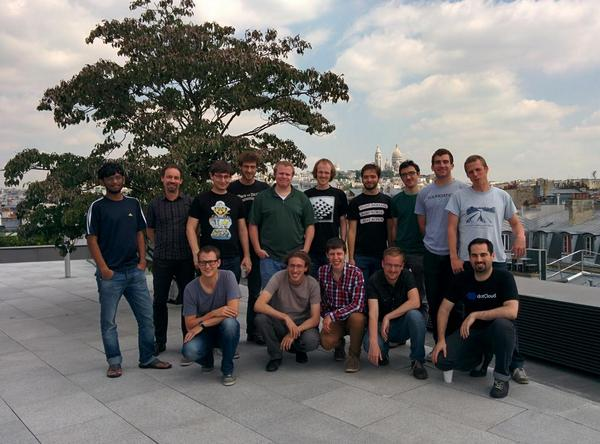
\includegraphics[width=0.7\textwidth]{scikit-learn-sprint.jpg}

\begin{small}
\structure{scikit-learn sprint 2014}
\end{small}
\end{center}

    
\end{frame}



\begin{frame}[allowframebreaks]%in case more than 1 slide needed
\frametitle{References} 

{\footnotesize
    \bibliographystyle{apalike}
    \bibliography{references}
}
\end{frame}




\end{document}

